\documentclass[a4paper]{article}
\usepackage{graphicx} % Required for inserting images
\usepackage{physics}
\usepackage[margin=2cm]{geometry}
\usepackage[italian]{babel}
\usepackage{siunitx}
\usepackage{float}
\usepackage{hyperref}
\usepackage[shortlabels]{enumitem}
\sisetup{separate-uncertainty=true}
\hypersetup{hidelinks, linktoc=all}
\usepackage{subfig}
\usepackage{changepage}
\usepackage[toc,page]{appendix}
\usepackage{breqn}
\usepackage{ntheorem}

\sisetup{per-mode=symbol}

\title{\textbf{Lenti}}
\author{Agostino Luca, Cafaro Alessandro, Gili Francesco, Gros Jacques Matteo\\ Turno AII - Gruppo 7\\A.A. 2024-2025}
\date{\today}

\begin{document}
    
\maketitle

\tableofcontents
\newpage

\section{Obiettivi della misura}
    Verificare la validità delle leggi sulle lenti sottili, misurandone le proprietà geometriche; in particolare:
    \begin{enumerate}
        \item Ricavare la distanza focale e l'ingrandimento di una lente biconvessa
        \item Ricavare la distanza focale di una lente piano-convessa
        \item Ricavare la distanza focale di una lente divergente
        \item Misurare la posizione dell'immagine di un sistema di due lenti convergenti non a contatto.
    \end{enumerate}
\section{Apparato sperimentale}
    \begin{itemize}
        \item Banco ottico (sensibilità: \SI{1}{\mm})
        \item Proiettore con illuminazione regolabile
        \item Diapositiva da proiettare
        \item Lenti di diverso tipo: biconvessa, piano-convessa, biconcava
        \item Schermo per visualizzare l'immagine
        \item Calibro (sensibilità: \SI{0.05}{\mm})
    \end{itemize}
\section{Presa dati}
    \subsection{Lente biconvessa}\label{sec:biconvessa}
        Abbiamo fissato la lente biconvessa su un supporto posto a distanza $p=\SI{0.140(2)}{\m}$. Successivamente abbiamo compiuto 70 misure ripetute della posizione dell'immagine, spostando lo schermo finché questa non risultasse nitida, con l'accortezza di alternare destra e sinistra come direzioni di avvicinamento.
        %Dati.

        Ci aspettiamo che i due fuochi abbiano la stessa distanza dalla lente; l'abbiamo quindi ruotato di $\pi$ e ripetuto le misure utilizzando la stessa procedura e le medesime accortezze.

        Per entrambe le lenti abbiamo poi calcolato l'ingrandimento come il rapporto tra la distanza di due punti distinti sullo schermo e degli stessi sulla diapositiva.
        %Dati
        
    \subsection{Lente piano-convessa}    
    Abbiamo ripetuto le precedenti misurazioni su una lente convergente piano-convessa mantenendo inalterato il numero di misure e la procedura utilizzata.
    
    \subsection{Lente biconcava}
    Riutilizzando la lente biconvessa della Sezione \ref{sec:biconvessa}, costruiamo un sistema ottico formato da quest'ultima e da una lente negativa biconcava, montandole in modo che siano il più possibile vicine tra loro. Poniamo le due lenti a distanza $p$ dall'oggetto, ed esattamente nello stesso modo descritto precedentemente, misuriamo ripetutamente $q$.
    
    \subsection{Sistema di lenti}
    Utilizzando due lenti convergenti disposte non a contatto, abbiamo misurato 10 volte il valore di $q_2$, ossia la distanza dalle lenti che rende nitida l'immagine sullo schermo.
\section{Analisi dati}
    \subsection{Lente biconvessa}
    Poiché abbiamo compiuto $N=70$ misure ripetute della stessa grandezza, ci aspettiamo che i dati si distribuiscano secondo un andamento gaussiano. Abbiamo dunque eseguito un fit dell'istogramma delle frequenze assolute dei dati.
    \begin{figure}[H]
    	\centering
    	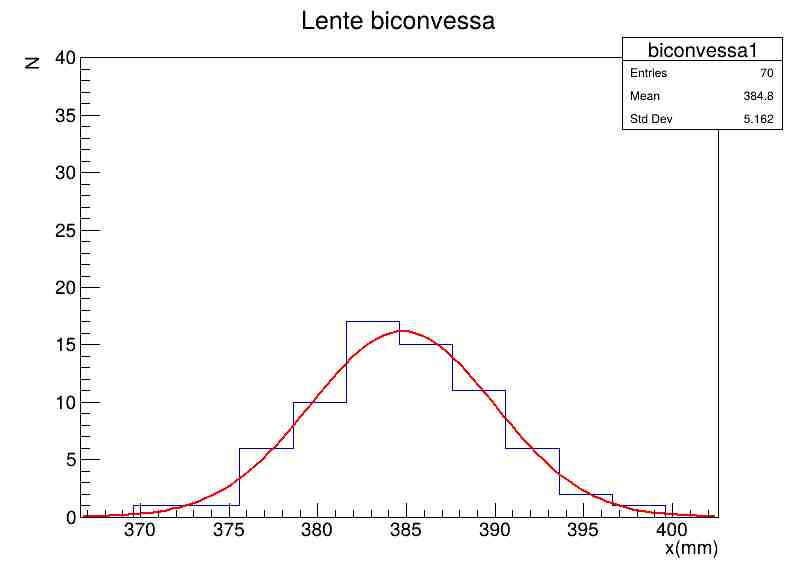
\includegraphics[width=0.75\linewidth]{histo1.jpg}
    	\caption{Lente biconvessa}
    	\label{fig:biconvessa}
    \end{figure}
    Di seguito riportiamo il test del $\chi^2$, con un livello di significatività del $5\%$:
    \[
    H_0: \text{la distribuzione gaussiana ben descrive quella dei dati sperimentali.}
    \]
    \begin{table}[H]
    	\centering
    	\begin{tabular}{|c|c|}
    		\hline
    		$\chi^2$ & 1.942 \\
    		$\nu$ & 9 \\
    		$\chi^2_c$ & 16.919\\
    		$\chi^2_s$ & 3.325\\ \hline
    	\end{tabular}
    	\label{tab:chi-quadro-biconvessa}
    \end{table}
    $\chi^2\leq\chi^2_s<\chi^2_c$, questo significa che 
    \subsection{Lente biconcava}
    \subsection{Sistema di lenti}
\section{Risultati e osservazioni conclusive}
    \subsection{Lente biconvessa}
    \subsection{Lente biconcava}
    \subsection{Sistema di lenti}
\begin{appendices}
    \section{Dati}
    \section{Calcoli}
\end{appendices}
\end{document}
